\documentclass[11pt,a4paper,english]{article}
    \usepackage[latin1]{inputenc}
    \usepackage{amsmath,amsfonts,amssymb}
    \usepackage{enumitem}
    \usepackage{fullpage}
    \usepackage{graphicx}
    \usepackage{tabto}
    \usepackage{etoolbox}
    \usepackage{hyperref}
    \usepackage{minted}
    \usepackage{parskip}
    \usepackage[title]{appendix}
    \graphicspath{ {./} }

    \title{Bayesian Data Analysis - Assignment 3}
    \author{}

    \begin{document}
      \maketitle
      \definecolor{bg}{rgb}{0.95,0.95,0.95}

      \begin{enumerate}
        \item \textit{Inference for normal mean and deviation.}
          \begin{enumerate}[label=\alph*.]
            \item \textit{What can you say about the unknown $\mu$?}\\
              To answer to the questions it would be reasonable to plot the probability
              distribution function. But before plotting the graph we have to follow the formulas
              and some conventions. For instance to plot the $pdf$ we have to calculate the
              degree of freedom, which is $n-1$; the location: $np.mean(data)$ and the
              estimated variance: $stats.tvar(data)/n$. These are important components for
              computing $\mu$:
              \begin{minted}[bgcolor=bg,fontsize=\small,autogobble]{python}
                y_range = stats.t.pdf(
                    x=x_range,
                    df=n-1,
                    loc=estimated_mean,
                    scale=estimated_variance/n
                )
              \end{minted}

              It looks like this:\\
              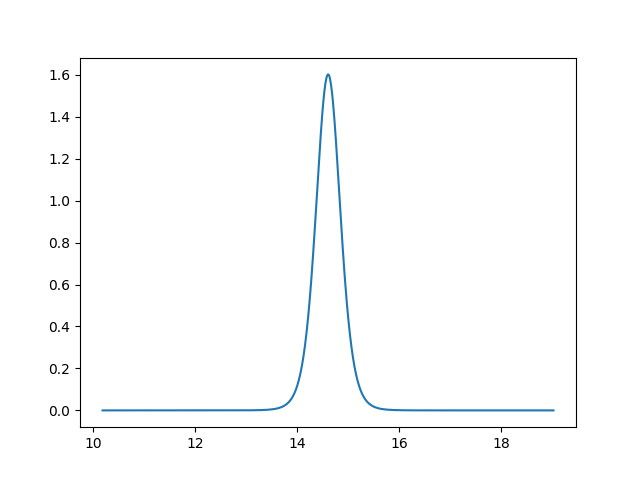
\includegraphics[width=10cm]{3_1_a_mean_student_distribution.png}

              From that we can say that $\mu$ is concentrated between \textbf{intervals [14.054, 15.168]}
              and has an \textbf{average hardness of 14.611} with estimated \textbf{variance 2.173} and
              estimated \textbf{standard deviation 1.474}.

              \begin{minted}[bgcolor=bg,fontsize=\small,autogobble]{bash}
                $ intervals: [14.054, 15.168]
                $ estimated mean: 14.611
                $ estimated variance: 2.173
                $ estimated standard deviation: 1.474
              \end{minted}
              Please see \textit{Appendix A Source code for 1 "a" and "b"} for reference.

            \item \textit{
              What can you say about the hardness of the next windshield coming
              from the production line before actually measuring the hardness?}\\
              We can say with the \textbf{95\% confidence} that the hardness of the next
              windshield coming from the production line will be between \textbf{intervals [14.054, 15.168]}.
              The same formula as in $a$ can be applied to plot it:\\
              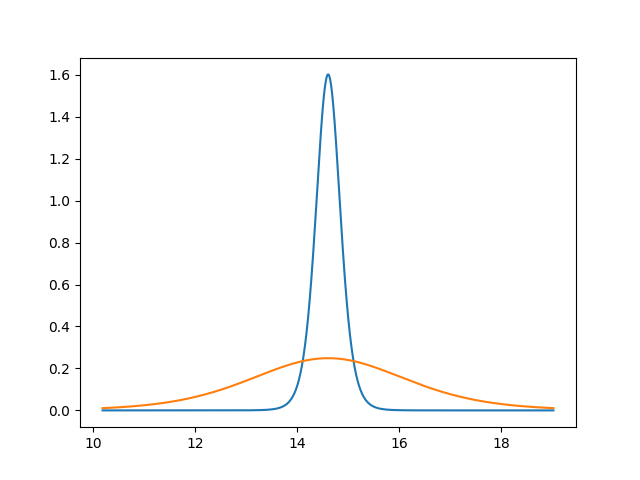
\includegraphics[width=10cm]{3_1_b_posterior_mean.png}
          \end{enumerate}

        \item \textit{Inference for difference between proportions:}
          \begin{enumerate}[label=\alph*.]
            \item \textit{Compute the point and interval estimates and plot the histograms:}\\
              The histogram can be plotted by following the given $(p_1/(1-p_1))/(p_0/(1-p_0))$ and using
              and python "magic" packages:

              \begin{minted}[bgcolor=bg,fontsize=\small,autogobble]{bash}
                p_control = stats.beta.rvs(control_alpha, control_beta, size=10000)
                p_treatment = stats.beta.rvs(treatment_alpha, treatment_beta, size=10000)
                odd_ratio = (p_treatment/(1-p_treatment))/(p_control/(1-p_control))
                plt.hist(odd_ratio, alpha=0.5, bins=40, ec='white')
              \end{minted}

              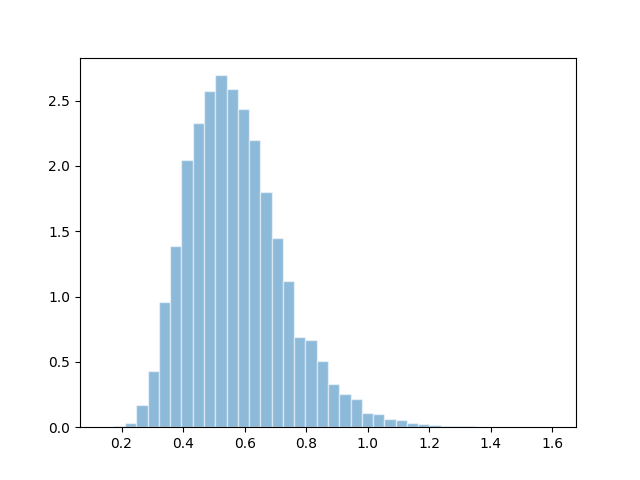
\includegraphics[width=10cm]{3_2_b_histog.png}

              \begin{minted}[bgcolor=bg,fontsize=\small,autogobble]{bash}
                $ Control central percentile 95%:  [0.043, 0.0785]
                $ Treatment central percentile 95%:  [0.0218, 0.0489]
                $ Control posterior mean:  0.0593
                $ Treatment posterior mean:  0.0338
              \end{minted}
              Please see \textit{Appendix B  Source code for 2 "a" and "b"} for reference.

            \item \textit{Discuss the sensitivity of your inference to your choice
              of prior density with a couple of sentences:}\\
              Based on the plotted graph that depicts the control group and treatment group,
              we can conclude that the treatment does not have a big positive impact.

              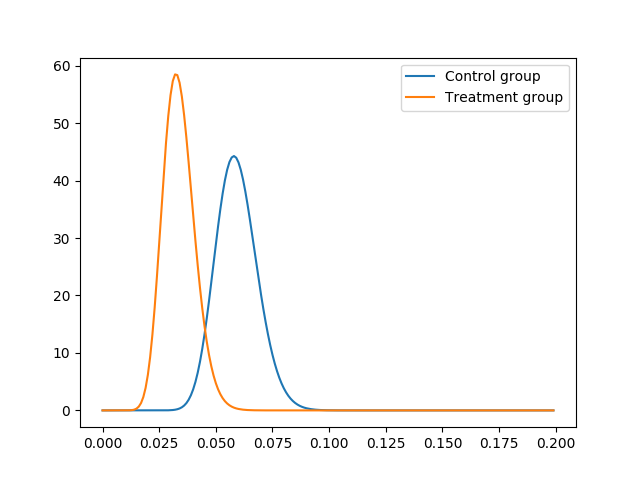
\includegraphics[width=10cm]{3_2_a_control_beta.png}

              Since we have chosen an uninformative prior, it does not impact on our
              inference.
          \end{enumerate}

        \item \textit{Inference for difference between normal means:}\\
          For this example we can use $uninformative priors$ and use exactly the same formula
          as for $3.1\ "a",\ "b"$. The only issue is that we have to optimize our code and
          reuse it to calculate both $mu_1$ and $mu_2$. That optimization can then help us to
          calculate the values quickly.
          \begin{minted}[bgcolor=bg,fontsize=\small,autogobble]{bash}
            n_1, estimated_mean_1, estimated_variance_1, x_range_1, mu_1 = get_attributes(y1)
            n_2, estimated_mean_2, estimated_variance_2, x_range_2, mu_2 = get_attributes(y2)
          \end{minted}
          Please see \textit{Appendix C  Source code for 3 "a" and "b"} for reference.

          \begin{enumerate}[label=\alph*.]
            \item The histogram of $\mu_d$ = $\mu_1$ - $\mu_2$ looks like this:

              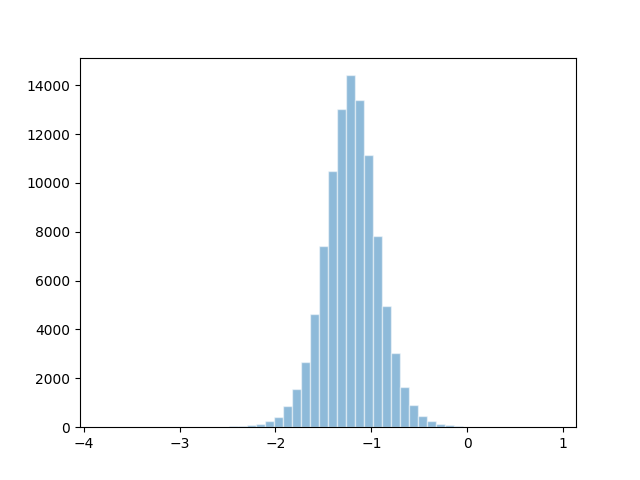
\includegraphics[width=10cm]{3_3_a_histogram.png}

            \item \textit{Are the means the same? Explain your reasoning with a couple of sentences.}\\
              No they are not the same. Since 99.942\% of the points are below 0, then we can conclude that they are not the same.

              \begin{minted}[bgcolor=bg,fontsize=\small,autogobble]{bash}
                $ Intervals -1.7847 -0.6424
                $ Percentile of m < 0: 99.939 %
              \end{minted}
          \end{enumerate}
      \end{enumerate}
      \begin{appendices}
        \section{Source code for 1 "a" and "b"}
        \begin{minted}[bgcolor=bg,linenos,fontsize=\small,autogobble]{python}
          import matplotlib
          matplotlib.use('TkAgg')
          from math import sqrt
          from scipy import stats
          import matplotlib.pyplot as plt
          import numpy as np

          data = [
              13.357,
              14.928,
              14.896,
              15.297,
              14.82,
              12.067,
              14.824,
              13.865,
              17.447,
          ]
          n = len(data)
          estimated_mean = np.mean(data)
          estimated_variance = stats.tvar(data)
          x_range = np.arange(
              estimated_mean - 3 * sqrt(estimated_variance),
              estimated_mean + 3 * sqrt(estimated_variance),
              0.01
          )

          '''
          a) What can you say about the unknown μ?
          '''
          y_range = stats.t.pdf(
              x=x_range,
              df=n-1,
              loc=estimated_mean,
              scale=estimated_variance/n
          )
          intervals = stats.t.interval(
              0.95,
              df=n-1,
              loc=estimated_mean,
              scale=estimated_variance/n
          )
          low, up = intervals
          print('a)')
          print('-- intervals:', [round(low, 3), round(up, 3)])
          print('-- estimated mean:', round(estimated_mean, 3))
          print('-- estimated variance:', round(estimated_variance, 3))
          print('-- estimated standard deviation:', round(sqrt(estimated_variance), 3))
          figure = plt.plot(x_range, y_range)
          plt.savefig('./ex3/report/3_1_a_mean_student_distribution.png')

          '''
          b)
          '''
          std_y = np.std(data, ddof=1)
          scale = sqrt(1 + 1/n) * std_y
          y_posterior_range = stats.t.pdf(
              x=x_range,
              df=n-1,
              loc=estimated_mean,
              scale=scale
          )
          figure = plt.plot(x_range, y_posterior_range)
          plt.savefig('./ex3/report/3_1_b_posterior_mean.png')
        \end{minted}
      \end{appendices}

      \begin{appendices}
        \section{Source code for 2 "a" and "b"}
        \begin{minted}[bgcolor=bg,linenos,fontsize=\small,autogobble]{python}
          import matplotlib
          matplotlib.use('TkAgg')
          from scipy import stats
          import matplotlib.pyplot as plt
          import numpy as np

          x_range = np.arange(0, 0.2, 0.001)

          '''
          a)
          '''
          control = 674
          control_died = 39
          control_alpha = control_died + 1
          control_beta = control - control_alpha + 1
          control_posterior = control_alpha/control
          control_pdf = stats.beta.pdf(x_range, control_alpha, control_beta)
          control_pdf_line = plt.plot(x_range, control_pdf)

          treatment = 680
          treatment_died = 22
          treatment_alpha = treatment_died + 1
          treatment_beta = treatment - treatment_alpha + 1
          treatment_posterior = treatment_alpha/treatment
          treatment_pdf = stats.beta.pdf(x_range, treatment_alpha, treatment_beta)
          treatment_pdf_line = plt.plot(x_range, treatment_pdf)

          plt.legend(
              [*control_pdf_line, *treatment_pdf_line],
              ['Control group', 'Treatment group']
          )
          plt.savefig('./ex3/report/3_2_a_control_beta.png')
          plt.figure(0)

          '''
          b)
          '''
          p_control = stats.beta.rvs(control_alpha, control_beta, size=10000)
          p_treatment = stats.beta.rvs(treatment_alpha, treatment_beta, size=10000)
          odd_ratio = (p_treatment/(1-p_treatment))/(p_control/(1-p_control))

          plt.hist(odd_ratio, alpha=0.5, bins=40, ec='white')
          plt.savefig('./ex3/report/3_2_b_histog.png')
          plt.figure(0)

          '''
          intervals
          '''
          control_percentile_25 = np.percentile(p_control, q=2.5)
          control_percentile_95 = np.percentile(p_control, q=97.5)

          treatment_percentile_25 = np.percentile(p_treatment, q=2.5)
          treatment_percentile_95 = np.percentile(p_treatment, q=97.5)
          print('-----------')
          print(
              'Control central percentile 95%: ',
              [round(control_percentile_25, 4), round(control_percentile_95, 4)]
          )
          print(
              'Treatment central percentile 95%: ',
              [round(treatment_percentile_25, 4), round(treatment_percentile_95, 4)]
          )
          print('Control posterior mean: ', round(np.mean(control_posterior), 4))
          print('Treatment posterior mean: ', round(np.mean(treatment_posterior), 4))
        \end{minted}
      \end{appendices}

      \begin{appendices}
        \section{Source code for 3 "a" and "b"}
        \begin{minted}[bgcolor=bg,linenos,fontsize=\small,autogobble]{python}
          import matplotlib
          matplotlib.use('TkAgg')
          from math import sqrt
          import scipy
          from scipy import stats
          import matplotlib.pyplot as plt
          import numpy as np

          def get_attributes(data):
              n = len(data)
              estimated_mean = np.mean(data)
              estimated_variance = stats.tvar(data)
              x_range = np.arange(
                  estimated_mean - 3 * sqrt(estimated_variance),
                  estimated_mean + 3 * sqrt(estimated_variance),
                  0.01
              )
              mu = stats.t.pdf(
                  x=x_range,
                  df=n-1,
                  loc=estimated_mean,
                  scale=estimated_variance/n
              )
              return [n, estimated_mean, estimated_variance, x_range, mu]

          y1 = [13.357,14.928,14.896,15.297,14.82,12.067,14.824,13.865,17.447]
          y2 = [15.98,14.206,16.011,17.25,15.993,15.722,17.143,15.23,15.125,
            16.609,14.735,15.881,15.789]
          n_1, estimated_mean_1, estimated_variance_1, x_range_1, mu_1 = get_attributes(y1)
          n_2, estimated_mean_2, estimated_variance_2, x_range_2, mu_2 = get_attributes(y2)

          mu_1_samples = stats.t.rvs(
            df=n_1-1, loc=estimated_mean_1, scale=estimated_variance_1/n_1, size=100000
          )
          mu_2_samples = stats.t.rvs(
            df=n_2-1, loc=estimated_mean_2, scale=estimated_variance_2/n_2, size=100000
          )
          mu_diff = mu_1_samples - mu_2_samples

          plt.hist(mu_diff, bins=50, ec='white',  alpha=0.5)
          plt.savefig('./ex3/report/3_3_a_histogram.png')
          print(
            'Intervals',
            round(np.percentile(mu_diff, 2.5), 4),
            round(np.percentile(mu_diff, 97.5), 4)
          )

          '''
          b)
          '''
          print(stats.percentileofscore(mu_diff, 0), '%')
        \end{minted}
      \end{appendices}
  \end{document}
